% ------------------------------------------------------------------------
% Architekturdokumentation (arc42) -- Einzeldatei
% eBay-Klon als Microservices-Architektur
%
% Selbstständig kompilierbar:  pdflatex arc42-dokumentation.tex
% (keine externen .tex-Dateien, keine externen Bilder noetig;
%  alle Diagramme sind als TikZ eingebettet)
% ------------------------------------------------------------------------
\documentclass[11pt,a4paper]{article}

\usepackage[top=2.5cm, bottom=2.5cm, left=2.8cm, right=2.8cm]{geometry}
\usepackage[utf8]{inputenc}
\usepackage[T1]{fontenc}
\usepackage{lmodern}
\usepackage{textcomp}
\usepackage{amsmath,amssymb}
\usepackage{microtype}
\usepackage{parskip}
\usepackage{xcolor}
\usepackage{graphicx}
\usepackage{longtable,booktabs,tabularx,array}
\usepackage{enumitem}
\usepackage{fancyhdr}
\usepackage{tikz}
\usetikzlibrary{shapes.geometric, arrows, positioning, arrows.meta}
\usepackage{hyperref}
\hypersetup{
  pdftitle={Architekturdokumentation -- eBay-Klon als Microservices-Architektur},
  hidelinks
}

% ------------------------------------------------------------------------
% Tabellen-Stil
% ------------------------------------------------------------------------
\colorlet{tableHeaderColor}{gray!25}
\colorlet{tableRowColor}{gray!14}
\newcommand{\tabellenkopf}{%
  \renewcommand{\arraystretch}{1.4}%
  \rowcolors{2}{tableRowColor}{white}%
}

\pagestyle{fancy}
\fancyhf{}
\fancyhead[R]{\small\thepage}
\renewcommand{\headrulewidth}{0.4pt}
\fancypagestyle{plain}{\fancyhf{}\fancyhead[R]{\small\thepage}}

\setcounter{secnumdepth}{3}
\setcounter{tocdepth}{2}

\begin{document}

% ========================================================================
% Titelblatt
% ========================================================================
\begin{titlepage}
\centering
\vspace*{\fill}
{\Huge\bfseries Architekturdokumentation}\\[8pt]
{\LARGE eBay-Klon als Microservices-Architektur}\\[20pt]
{\large Gruppe 5 -- Software-Architektur}\\[12pt]
Dominik Duken \quad Noah Preyer \quad Ilker T\"urk\\[8pt]
Juli 2026
\vspace*{\fill}
\end{titlepage}

\tableofcontents
\newpage

% ========================================================================
% 1. Einfuehrung und Ziele
% ========================================================================
\section{Einf\"uhrung und Ziele}

\subsection{Aufgabenstellung}

Im Modul Software-Architektur sollte ein Architekturstil anhand einer
Beispielanwendung umgesetzt und bewertet werden. Dazu wurde eine
Microservices-Architektur f\"ur eine E-Commerce-Plattform (eBay-Klon)
entwickelt.

Die Plattform eignet sich besonders als Beispielanwendung, da sich ihre
Funktionen klar in Bereiche wie Authentifizierung, Produktverwaltung,
Bestellabwicklung und Benachrichtigungen aufteilen lassen. Durch die
modulare Struktur kann das System leicht um weitere Funktionen und
Services erweitert werden.

\subsection{Kernfunktionen}

\begin{itemize}[leftmargin=1.5em, itemsep=2pt]
  \item Registrierung und Anmeldung mittels JWT
  \item Erstellen, Bearbeiten, L\"oschen und Suchen von Produkten
  \item Kaufabwicklung inklusive Bestellung und Statuswechsel
  \item E-Mail-Benachrichtigungen (Bestell-, Versand- und
        Lieferbest\"atigung)
\end{itemize}

\subsection{Qualit\"atsziele}

\begin{center}
\tabellenkopf
\begin{tabularx}{\linewidth}{
        >{\bfseries\raggedright\arraybackslash}p{0.25\linewidth}
        >{\raggedright\arraybackslash}X}
    \toprule
    \rowcolor{tableHeaderColor}
    Qualit\"atsziel & Beschreibung \\
    \midrule
    Modularit\"at &
    Fachliche Bereiche sind in eigenst\"andige Services aufgeteilt. \\
    Lose Kopplung &
    Kommunikation \"uber klar definierte REST-Schnittstellen und
    MQTT-Nachrichten. \\
    Skalierbarkeit &
    Einzelne Services k\"onnen unabh\"angig horizontal skaliert werden. \\
    Sicherheit &
    Authentifizierung und JWT-Validierung erfolgen zentral \"uber das
    API Gateway. \\
    Erweiterbarkeit &
    Neue Services k\"onnen \"uber bestehende Schnittstellen erg\"anzt
    werden. \\
    Fehlertoleranz &
    Der Ausfall eines einzelnen Services soll nicht das gesamte System
    beeintr\"achtigen. \\
    \bottomrule
\end{tabularx}
\end{center}

\subsection{Stakeholder}

\begin{itemize}[leftmargin=1.5em, itemsep=2pt]
  \item \textbf{Dozent:} bewertet Architekturstil, Dokumentation und
        Pr\"asentation.
  \item \textbf{Projektgruppe:} entwickelt, betreibt und erweitert die
        Plattform.
\end{itemize}

% ========================================================================
% 2. Randbedingungen
% ========================================================================
\section{Randbedingungen}

\begin{description}[leftmargin=1.5em, itemsep=2pt]
  \item[Freie Technologiewahl]
  Es gab keine Vorgabe f\"ur den Technologie-Stack. Diese Freiheit wurde
  bewusst genutzt, um die f\"ur Microservices typische
  Technologieoffenheit tats\"achlich zu erproben (polyglotter Stack aus
  Java/Spring Boot, Python/Flask und einem Astro-Frontend).
  \item[Lokale Ausf\"uhrbarkeit]
  Das gesamte System muss isoliert und auf einem normalen Computer
  startbar sein. Daraus folgt der Einsatz von Docker Compose anstelle
  einer Cloud-Umgebung.
  \item[Organisatorisch]
  Die Dokumentation ist als Gruppenarbeit entstanden und umfasst
  einschlie\ss{}lich Diagrammen 8--12 Seiten.
\end{description}

% ========================================================================
% 3. Kontextabgrenzung
% ========================================================================
\section{Kontextabgrenzung}

\subsection{Fachlicher Kontext}

Die Plattform wird von registrierten und nicht registrierten Benutzern
verwendet. Nicht registrierte Benutzer k\"onnen Produkte suchen, aufrufen
und sich registrieren. Registrierte Benutzer k\"onnen zus\"atzlich eigene
Produkte einstellen und Produkte kaufen. Nach einem erfolgreichen Kauf
wird eine Bestellbest\"atigung versendet.

Nach au\ss{}en tritt die Plattform als eine zusammenh\"angende Anwendung
auf. Die einzige Verbindung zu einem externen System besteht zum
E-Mail-Dienst (SMTP), der f\"ur den Versand der Bestellbest\"atigungen
verwendet wird.

\subsection{Technischer Kontext}

Der Zugriff erfolgt ausschlie\ss{}lich \"uber einen Webbrowser. Dieser
l\"adt das mit Astro umgesetzte Frontend, das \"uber HTTP-REST-Anfragen
mit dem API Gateway auf Port 8080 kommuniziert. Das API Gateway bildet
den zentralen Einstiegspunkt zu den internen Services. Die Kommunikation
zwischen den Services erfolgt \"uber REST (synchron) und MQTT
(asynchron).

\begin{center}
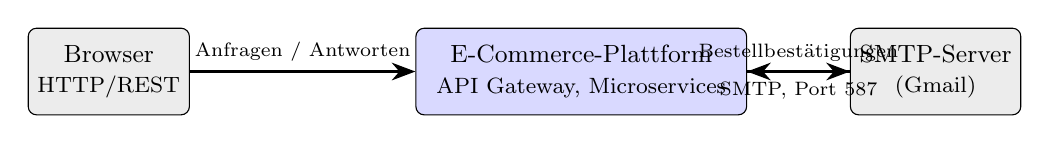
\begin{tikzpicture}[
    box/.style={rectangle, draw, rounded corners=3pt,
                minimum height=1.1cm, align=center, font=\small},
    ext/.style={box, fill=gray!15},
    arrow/.style={-{Stealth[length=3mm]}, thick}]
  \node[ext] (browser) at (0,0)
        {Browser\\\footnotesize HTTP/REST};
  \node[box, fill=blue!15, minimum width=4.2cm] (sys) at (6,0)
        {E-Commerce-Plattform\\\footnotesize API Gateway, Microservices};
  \node[ext] (smtp) at (10.5,0)
        {SMTP-Server\\\footnotesize (Gmail)};
  \draw[arrow] (browser) -- node[above, font=\scriptsize]
        {Anfragen / Antworten} (sys);
  \draw[arrow] (sys) -- node[above, font=\scriptsize]
        {Bestellbest\"atigungen} (smtp);
  \draw[arrow] (smtp) -- node[below, font=\scriptsize]
        {SMTP, Port 587} (sys);
\end{tikzpicture}
\captionof{figure}{Kontextdiagramm der E-Commerce-Plattform}
\end{center}

\subsubsection{Externe Schnittstellen}

\begin{center}
\tabellenkopf
\begin{tabularx}{\linewidth}{
        >{\bfseries\raggedright\arraybackslash}p{0.25\linewidth}
        >{\raggedright\arraybackslash}p{0.15\linewidth}
        >{\raggedright\arraybackslash}X}
    \toprule
    \rowcolor{tableHeaderColor}
    Gegenstelle & Richtung & Inhalt und Protokoll \\
    \midrule
    Nutzer \"uber Webbrowser &
    Bidirektional &
    Zugriff auf die Plattform \"uber HTTP/REST, z.\,B. f\"ur Anmeldung,
    Produktverwaltung und Kaufabwicklung. \\
    SMTP-Server (Gmail) &
    Ausgehend &
    Versand von Bestellbest\"atigungen \"uber SMTP mit STARTTLS auf
    Port 587. \\
    \bottomrule
\end{tabularx}
\end{center}

% ========================================================================
% 4. Loesungsstrategie
% ========================================================================
\section{L\"osungsstrategie}

Die Anwendung wurde als Microservice-Architektur umgesetzt. Die
wichtigsten L\"osungsans\"atze sind in Tabelle~\ref{tab:loesung}
zusammengefasst.

\begin{center}
\tabellenkopf
\begin{tabularx}{\linewidth}{
        >{\bfseries\raggedright\arraybackslash}p{0.22\linewidth}
        >{\raggedright\arraybackslash}p{0.38\linewidth}
        >{\raggedright\arraybackslash}X}
    \toprule
    \rowcolor{tableHeaderColor}
    Bereich & Umsetzung & Begr\"undung \\
    \midrule
    Systemaufteilung &
    Fachlich getrennte Microservices &
    Verbessert Modularit\"at und Erweiterbarkeit. \\
    Zugriff &
    Zentrales API Gateway mit JWT-Validierung &
    Einheitlicher und gesch\"utzter Einstiegspunkt. \\
    Kommunikation &
    REST f\"ur synchrone Aufrufe, MQTT f\"ur Ereignisse &
    Reduziert die Kopplung zwischen den Services. \\
    Persistenz &
    Database-per-Service (eigene PostgreSQL je Service) &
    Erzwingt lose Kopplung, keine geteilten Datenbanken. \\
    Technologien &
    Spring Boot, Flask, Astro und SolidJS &
    Geeignete Technologie je Komponente. \\
    Betrieb &
    Containerisierung mit Docker Compose &
    Vereinfacht Bereitstellung und Ausf\"uhrung. \\
    \bottomrule
\end{tabularx}
\end{center}

\begin{table}[ht]
  \centering
  \caption{Zentrale L\"osungsans\"atze}
  \label{tab:loesung}
\end{table}

% ========================================================================
% 5. Bausteinsicht
% ========================================================================
\section{Bausteinsicht}

\subsection{Level 1 -- Gesamtsystem}

Die Plattform besteht aus einem Frontend, einem zentralen API Gateway,
fachlich getrennten Microservices, einem MQTT-Broker und je einer
eigenen Datenbank pro Service.

\begin{center}
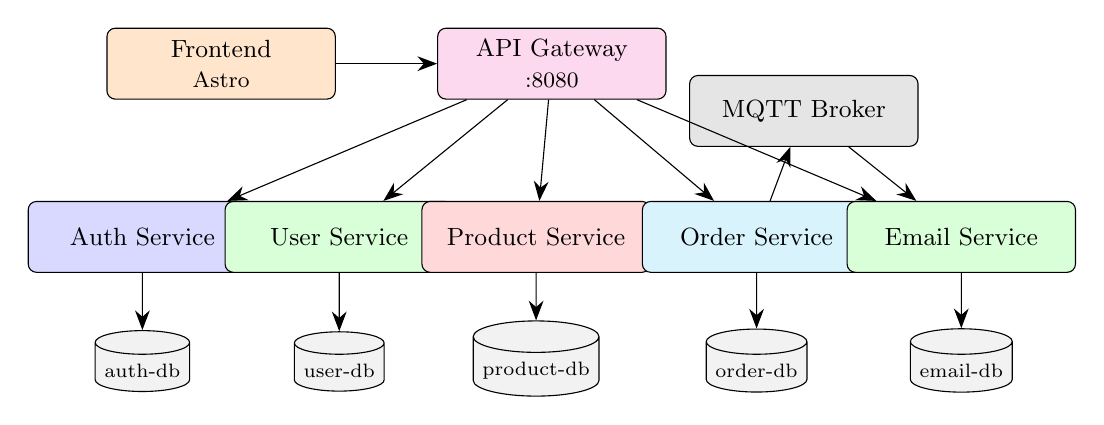
\begin{tikzpicture}[
    box/.style={rectangle, draw, rounded corners=3pt, align=center,
                font=\small, minimum width=2.9cm, minimum height=0.9cm},
    db/.style={cylinder, shape border rotate=90, aspect=0.25, draw,
               align=center, font=\scriptsize, fill=gray!10,
               minimum height=0.6cm},
    arrow/.style={-{Stealth[length=2.5mm]}, thin}]
  \node[box, fill=orange!20] (fe) at (0,0) {Frontend\\\footnotesize Astro};
  \node[box, fill=magenta!15] (gw) at (4.2,0) {API Gateway\\\footnotesize :8080};
  \node[box, fill=blue!15] (auth) at (-1,-2.2) {Auth Service};
  \node[box, fill=green!15] (user) at (1.5,-2.2) {User Service};
  \node[box, fill=red!15] (prod) at (4,-2.2) {Product Service};
  \node[box, fill=cyan!15] (order) at (6.8,-2.2) {Order Service};
  \node[box, fill=green!15] (email) at (9.4,-2.2) {Email Service};
  \node[box, fill=gray!20] (mqtt) at (7.4,-0.6) {MQTT Broker};
  \node[db] (dbauth) at (-1,-3.9) {auth-db};
  \node[db] (dbuser) at (1.5,-3.9) {user-db};
  \node[db] (dbprod) at (4,-3.9) {product-db};
  \node[db] (dborder) at (6.8,-3.9) {order-db};
  \node[db] (dbemail) at (9.4,-3.9) {email-db};
  \draw[arrow] (fe) -- (gw);
  \draw[arrow] (gw) -- (auth);
  \draw[arrow] (gw) -- (user);
  \draw[arrow] (gw) -- (prod);
  \draw[arrow] (gw) -- (order);
  \draw[arrow] (gw) -- (email);
  \draw[arrow] (order) -- (mqtt);
  \draw[arrow] (mqtt) -- (email);
  \draw[arrow] (auth) -- (dbauth);
  \draw[arrow] (user) -- (dbuser);
  \draw[arrow] (prod) -- (dbprod);
  \draw[arrow] (order) -- (dborder);
  \draw[arrow] (email) -- (dbemail);
\end{tikzpicture}
\captionof{figure}{Bausteinsicht (Level 1) der E-Commerce-Plattform}
\end{center}

\subsection{Bausteine}

\begin{center}
\tabellenkopf
\begin{tabularx}{\linewidth}{
        >{\bfseries\raggedright\arraybackslash}p{0.24\linewidth}
        >{\raggedright\arraybackslash}X}
    \toprule
    \rowcolor{tableHeaderColor}
    Baustein & Verantwortung \\
    \midrule
    Frontend &
    Stellt die Benutzeroberfl\"ache bereit und sendet Anfragen an das
    API Gateway. \\
    API Gateway &
    Zentraler Einstiegspunkt; validiert JWTs und leitet Anfragen an die
    zust\"andigen Services weiter. \\
    Auth Service &
    Registrierung, Anmeldung und Ausstellung der JWTs. \\
    User Service &
    Verwaltet die Daten der Benutzer. \\
    Product Service &
    Verwaltet Produktanzeigen; Funktionen zum Erstellen, Bearbeiten,
    L\"oschen und Suchen (3 Replikate hinter Nginx). \\
    Order Service &
    Verarbeitet K\"aufe und verwaltet die zugeh\"origen Bestellungen. \\
    Email Service &
    Erstellt und versendet Bestellbest\"atigungen \"uber den externen
    Mailserver. \\
    MQTT Broker &
    Verteilt asynchrone Ereignisse (Publish/Subscribe), z.\,B.
    \texttt{order/complete}. \\
    \bottomrule
\end{tabularx}
\end{center}

\subsection{Exemplarische Whitebox: Order Service}

Der Order Service ist als klassische Spring-Boot-Anwendung
(Controller $\rightarrow$ Service $\rightarrow$ Repository) aufgebaut.
\"Uber HTTP-Clients greift er auf den Product Service (Produktdetails),
den User Service (E-Mail-Adresse) und den Email Service zu; beim
Statuswechsel auf \texttt{PAID} publiziert er ein MQTT-Event
\texttt{order/complete}.

% ========================================================================
% 6. Laufzeitsicht
% ========================================================================
\section{Laufzeitsicht}

\subsection{Anmeldung}

\begin{enumerate}[leftmargin=1.5em, itemsep=2pt]
  \item Der Benutzer sendet seine Anmeldedaten \"uber das Frontend.
  \item Das API Gateway leitet die Anfrage an den Auth Service weiter.
  \item Der Auth Service pr\"uft die Zugangsdaten und erstellt ein JWT
        (HS256, 60~Minuten Laufzeit).
  \item Das Token wird an den Benutzer zur\"uckgegeben und von diesem
        in Folgerequests mitgeschickt.
\end{enumerate}

\subsection{Kauf eines Produkts}

\begin{enumerate}[leftmargin=1.5em, itemsep=2pt]
  \item Der Benutzer startet den Kauf \"uber das Frontend.
  \item Das API Gateway validiert das JWT und leitet die Anfrage an den
        Product Service weiter (\texttt{POST /products/bulk-buy}).
  \item Der Product Service reserviert alle Artikel
        (\texttt{markAllAsSold}).
  \item Der Order Service legt die Bestellung an und holt je Artikel
        Titel und Preis beim Product Service.
  \item Nach erfolgreicher Bezahlung wechselt die Bestellung auf
        \texttt{PAID}; der Order Service publiziert das MQTT-Event
        \texttt{order/complete}.
  \item Der Email Service konsumiert das Event, rendert das Template und
        versendet die Bestellbest\"atigung per SMTP.
\end{enumerate}

Bei einem Fehler setzt der Product Service die Artikel per
\texttt{markAllAsAvailable} zur\"uck \textbf{(kompensierende
Transaktion)} -- es existiert kein verteilter Transaction Manager.

% ========================================================================
% 7. Verteilungssicht
% ========================================================================
\section{Verteilungssicht}

Das Gesamtsystem wird mittels Docker Compose orchestriert. F\"ur jeden
Service existiert eine eigene Compose-Datei, die \"uber
\texttt{include} im Root-\texttt{docker-compose.yml} zusammengef\"uhrt
wird. Tabelle~\ref{tab:verteilung} zeigt die Container \"Ubersicht.

\begin{center}
\tabellenkopf
\begin{tabularx}{\linewidth}{
        >{\bfseries\raggedright\arraybackslash}p{0.28\linewidth}
        >{\raggedright\arraybackslash}p{0.16\linewidth}
        >{\raggedright\arraybackslash}p{0.14\linewidth}
        >{\raggedright\arraybackslash}X}
    \toprule
    \rowcolor{tableHeaderColor}
    Container & Port (Host) & Replikate & Netzwerk \\
    \midrule
    API Gateway & 8080 & 1 & frontend \\
    Auth Service & 8081 & 1 & frontend \\
    User Service & 8082 & 1 & frontend \\
    Product Service & 8083 & 3 (hinter Nginx) & frontend \\
    Nginx (Product) & 8089 & 1 & frontend \\
    Order Service & 8087 & 1 & frontend \\
    Email Service & 8084 & 1 & frontend \\
    Frontend & 4321 & 1 & frontend \\
    MQTT Broker & 1883 & 1 & frontend \\
    PostgreSQL (je Service) & --- & je 1 & frontend \\
    \bottomrule
\end{tabularx}
\end{center}

\subsection{Skalierung}

Der Product Service wird horizontal auf drei Replikate skaliert. Ein
Nginx-Reverse-Proxy verteilt die Anfragen im Round-Robin-Verfahren. Da
der Service zustandslos ist (keine Session, keine lokalen Dateien), ist
dies ohne Migrationseffekte m\"oglich.

% ========================================================================
% 8. Querschnittliche Konzepte
% ========================================================================
\section{Querschnittliche Konzepte}

\subsection{Sicherheit}

\begin{itemize}[leftmargin=1.5em, itemsep=2pt]
  \item \textbf{JWT-Ausstellung:} Auth Service signiert Tokens mit
        HS256 und einem Secret.
  \item \textbf{JWT-Validierung:} Im API Gateway als \texttt{GlobalFilter}
        -- jeder gesch\"utzte Request wird gepr\"uft.
  \item \textbf{\"Offentliche Endpunkte:} \texttt{/auth/**},
        \texttt{GET /products/**}, \texttt{GET /image/**}.
  \item \textbf{Identit\"atsweitergabe:} Das Gateway setzt einen
        \texttt{X-User-Id}-Header f\"ur Downstream-Services.
\end{itemize}

\subsection{Kommunikation}

\begin{description}[leftmargin=1.5em, itemsep=2pt]
  \item[REST (synchron)] F\"ur Abfragen und Kommandos, bei denen eine
        sofortige Antwort n\"otig ist (Produktdetails, Bestellanlage).
  \item[MQTT (asynchron, Publish/Subscribe)] F\"ur
        E-Mail-Benachrichtigungen: Der Order Service publiziert
        \texttt{order/complete} an den Mosquitto-Broker, der Email
        Service konsumiert das Event. Dies entkoppelt die Services -- der
        Email Service kann ausfallen, ohne den Bestellfluss zu blockieren.
\end{description}

\subsection{Persistenz}

Jeder Service besitzt eine eigene PostgreSQL-Instanz
(Database-per-Service). Dies erzwingt lose Kopplung:
service\"ubergreifende Abfragen erfolgen \"uber REST-Aufrufe, nicht \"uber
Datenbank-Joins. Fremdreferenzen werden als einfache IDs abgebildet.

\subsection{Polyglotter Tech-Stack}

\begin{center}
\tabellenkopf
\begin{tabularx}{\linewidth}{
        >{\bfseries\raggedright\arraybackslash}p{0.3\linewidth}
        >{\raggedright\arraybackslash}X}
    \toprule
    \rowcolor{tableHeaderColor}
    Service & Technologie \\
    \midrule
    API Gateway & Java 17, Spring Cloud Gateway \\
    Auth Service & Python, Flask \\
    User Service & Java 17, Spring Boot 3 \\
    Product Service & Java 17, Spring Boot 3 \\
    Order Service & Java 17, Spring Boot 3 \\
    Email Service & Python, Flask \\
    Frontend & Astro, SolidJS, Node.js \\
    \bottomrule
\end{tabularx}
\end{center}

% ========================================================================
% 9. Architekturentscheidungen (ADRs)
% ========================================================================
\section{Architekturentscheidungen (ADRs)}

\begin{center}
\tabellenkopf
\begin{tabularx}{\linewidth}{
        >{\bfseries\raggedright\arraybackslash}p{0.3\linewidth}
        >{\raggedright\arraybackslash}p{0.33\linewidth}
        >{\raggedright\arraybackslash}X}
    \toprule
    \rowcolor{tableHeaderColor}
    Entscheidung & Kontext & Konsequenz \\
    \midrule
    ADR-1: Microservices &
    Demonstration der Microservice-Eigenschaften &
    H\"ohere Betriebskomplexit\"at, daf\"ur lose Kopplung. \\
    ADR-2: API Gateway &
    Einheitlicher Einstiegspunkt f\"ur Sicherheit und Routing &
    Single Point of Failure, aber zentrale Kontrolle. \\
    ADR-3: MQTT f\"ur E-Mails &
    Asynchrone Kommunikation demonstrieren, Ausfalltoleranz &
    Email-Ausfall blockiert Bestellung nicht. \\
    ADR-4: Database-per-Service &
    Vermeidung geteilter Datenbanken &
    Keine service\"ubergreifenden Joins m\"oglich. \\
    ADR-5: Polyglotter Stack &
    Technologieunabh\"angigkeit demonstrieren &
    H\"ohere Einarbeitungszeit, aber bewusste Entscheidung. \\
    ADR-6: Replikation Product Service &
    Horizontale Skalierung demonstrieren &
    Nginx als zus\"atzliche Infrastrukturkomponente. \\
    ADR-7: Kompensierende Transaktion &
    Kein verteilter Transaction Manager &
    Manuelle R\"uckabwicklung bei Fehlern. \\
    \bottomrule
\end{tabularx}
\end{center}

% ========================================================================
% 10. Qualitaetsanforderungen
% ========================================================================
\section{Qualit\"atsanforderungen}

\subsection{Qualit\"atsszenarien}

\begin{description}[leftmargin=1.5em, itemsep=4pt]
  \item[Szenario 1 -- Ausfalltoleranz]
  \emph{Der Email Service f\"allt aus.} Bestellungen werden weiterhin
  angenommen und gespeichert. Die E-Mail-Zustellung erfolgt erst nach
  Wiederherstellung des Services (lose Kopplung durch MQTT).
  \item[Szenario 2 -- Lastspitze]
  \emph{Viele Nutzer browsen gleichzeitig Produkte.} Drei Replikate des
  Product Service teilen sich die Last \"uber den Nginx-Load-Balancer.
  \item[Szenario 3 -- Unabh\"angiges Deployment}
  \emph{Ein neuer Service (z.\,B. Rating Service) soll hinzugef\"ugt
  werden.} Keine \"Anderung an bestehenden Services n\"otig -- neues
  Routing im Gateway, neue Docker-Compose-Datei.
\end{description}

% ========================================================================
% 11. Risiken und technische Schulden
% ========================================================================
\section{Risiken und technische Schulden}

\begin{description}[leftmargin=1.5em, itemsep=4pt]
  \item[Kein zentrales Logging/Monitoring]
  Es existiert keine Correlation-ID \"uber Services hinweg; die
  Fehlersuche im verteilten System ist erschwert.
  \item[Gateway als Single Point of Failure]
  F\"allt das API Gateway aus, ist das gesamte System nicht erreichbar.
  Kein Failover-Mechanismus vorgesehen.
  \item[Zyklische Abh\"angigkeit]
  Product Service $\leftrightarrow$ Order Service: Der Product Service
  ruft den Order Service beim Kauf auf, der Order Service holt
  Produktdetails beim Product Service.
  \item[Secrets im Klartext]
  JWT-Secret und SMTP-Zugangsdaten liegen unverschl\"usselt in den
  Docker-Compose-Dateien.
  \item[ID-Typ-Inkonsistenz]
  Auth- und User Service verwenden UUIDs, Product- und Order Service
  Long-IDs. Die \texttt{X-User-Id}-Kette ist damit aktuell nicht
  durchg\"angig funktionsf\"ahig.
\end{description}

% ========================================================================
% 12. Glossar
% ========================================================================
\section{Glossar}

\begin{center}
\tabellenkopf
\begin{tabularx}{\linewidth}{
        >{\bfseries\raggedright\arraybackslash}p{0.3\linewidth}
        >{\raggedright\arraybackslash}X}
    \toprule
    \rowcolor{tableHeaderColor}
    Begriff & Definition \\
    \midrule
    API Gateway &
    Zentraler Einstiegspunkt, routet Anfragen an die entsprechenden
    Services. \\
    JWT &
    JSON Web Token -- tokenbasiertes Authentifizierungsverfahren. \\
    MQTT &
    Message Queue Telemetry Transport -- asynchrones
    Publish/Subscribe-Protokoll. \\
    Database-per-Service &
    Architekturmuster: jeder Service besitzt eine eigene Datenbank. \\
    Polyglotter Stack &
    Verwendung verschiedener Programmiersprachen und Frameworks
    innerhalb eines Systems. \\
    Kompensierende Transaktion &
    Manuelles R\"uckg\"angigmachen einer vorherigen Aktion bei
    Fehlschlag. \\
    \bottomrule
\end{tabularx}
\end{center}

\end{document}
